%%%%%%%%%%%%%%%%%%%%%%%%%%%%%%%%%%%%%%%%%
% Beamer Presentation
% LaTeX Template
% Version 1.0 (10/11/12)
%
% This template has been downloaded from:
% http://www.LaTeXTemplates.com
%
% License:
% CC BY-NC-SA 3.0 (http://creativecommons.org/licenses/by-nc-sa/3.0/)
%
%%%%%%%%%%%%%%%%%%%%%%%%%%%%%%%%%%%%%%%%%

%----------------------------------------------------------------------------------------
%	PACKAGES AND THEMES
%----------------------------------------------------------------------------------------

\documentclass{beamer}

\mode<presentation> {

% The Beamer class comes with a number of default slide themes
% which change the colors and layouts of slides. Below this is a list
% of all the themes, uncomment each in turn to see what they look like.

%\usetheme{default}
%\usetheme{AnnArbor}
%\usetheme{Antibes}
%\usetheme{Bergen}
%\usetheme{Berkeley}
%\usetheme{Berlin}
%\usetheme{Boadilla}
\usetheme{CambridgeUS}
%\usetheme{Copenhagen}
%\usetheme{Darmstadt}
%\usetheme{Dresden}
%\usetheme{Frankfurt}
%\usetheme{Goettingen}
%\usetheme{Hannover}
%\usetheme{Ilmenau}
%\usetheme{JuanLesPins}
%\usetheme{Luebeck}
%\usetheme{Madrid}
%\usetheme{Malmoe}
%\usetheme{Marburg}
%\usetheme{Montpellier}
%\usetheme{PaloAlto}
%\usetheme{Pittsburgh}
%\usetheme{Rochester}
%\usetheme{Singapore}
%\usetheme{Szeged}
%\usetheme{Warsaw}

% As well as themes, the Beamer class has a number of color themes
% for any slide theme. Uncomment each of these in turn to see how it
% changes the colors of your current slide theme.

%\usecolortheme{albatross}
%\usecolortheme{beaver}
%\usecolortheme{beetle}
%\usecolortheme{crane}
%\usecolortheme{dolphin}
%\usecolortheme{dove}
%\usecolortheme{fly}
%\usecolortheme{lily}
%\usecolortheme{orchid}
%\usecolortheme{rose}
\usecolortheme{seagull}
%\usecolortheme{seahorse}
%\usecolortheme{whale}
%\usecolortheme{wolverine}

%\setbeamertemplate{footline} % To remove the footer line in all slides uncomment this line
%\setbeamertemplate{footline}[page number] % To replace the footer line in all slides with a simple slide count uncomment this line

%\setbeamertemplate{navigation symbols}{} % To remove the navigation symbols from the bottom of all slides uncomment this line
}



\newcommand\Fontvi{\fontsize{6}{7.2}\selectfont}
\newcommand\Fontvii{\fontsize{7}{8.2}\selectfont}
\newcommand\Fontviii{\fontsize{8}{9.2}\selectfont}
\newcommand\Fontviiii{\fontsize{9}{10.2}\selectfont}

\usepackage{graphicx} % Allows including images
\usepackage{booktabs} % Allows the use of \toprule, \midrule and \bottomrule in tables

%----------------------------------------------------------------------------------------
%	TITLE PAGE
%----------------------------------------------------------------------------------------

\title[Drawdown project]{Monthly Presentation of Drawdown project} % The short title appears at the bottom of every slide, the full title is only on the title page

\author{Boying Gong, Xinyue Zhou} % Your name
\institute[UC Berkeley] % Your institution as it will appear on the bottom of every slide, may be shorthand to save space
{
University of California, Berkeley \\ % Your institution for the title page
\medskip
\textit{jorothy\_gong@berkeley.edu \\}
\textit{xinyue233@berkeley.edu} % Your email address
}
\date{\today} % Date, can be changed to a custom date

\begin{document}

\begin{frame}
\titlepage % Print the title page as the first slide
\end{frame}

\begin{frame}
\frametitle{Overview} % Table of contents slide, comment this block out to remove it
\tableofcontents % Throughout your presentation, if you choose to use \section{} and \subsection{} commands, these will automatically be printed on this slide as an overview of your presentation
\end{frame}

%----------------------------------------------------------------------------------------
%	PRESENTATION SLIDES
%----------------------------------------------------------------------------------------

%------------------------------------------------
\section{Maximum drawdown distribution and CED}
%------------------------------------------------

%------------------------------------------------
\section{Regime switching models}
%------------------------------------------------

%------------------------------------------------
\section{Time Series – ARMA model}
%------------------------------------------------
\subsection{Motivations}
\begin{frame}
\frametitle{Motivations}
\Fontviii
\begin{columns}[c]
\column{.35\textwidth} % Left column and width
\begin{enumerate}
\item Find a correct model to characterize the returns of financial assets. 
\item Check the relationship between serial correlations (here we use $\kappa(1)$) and risk measurements.
\end{enumerate}

\column{.6\textwidth} % Right column and width
\begin{figure}[h]
\centering 
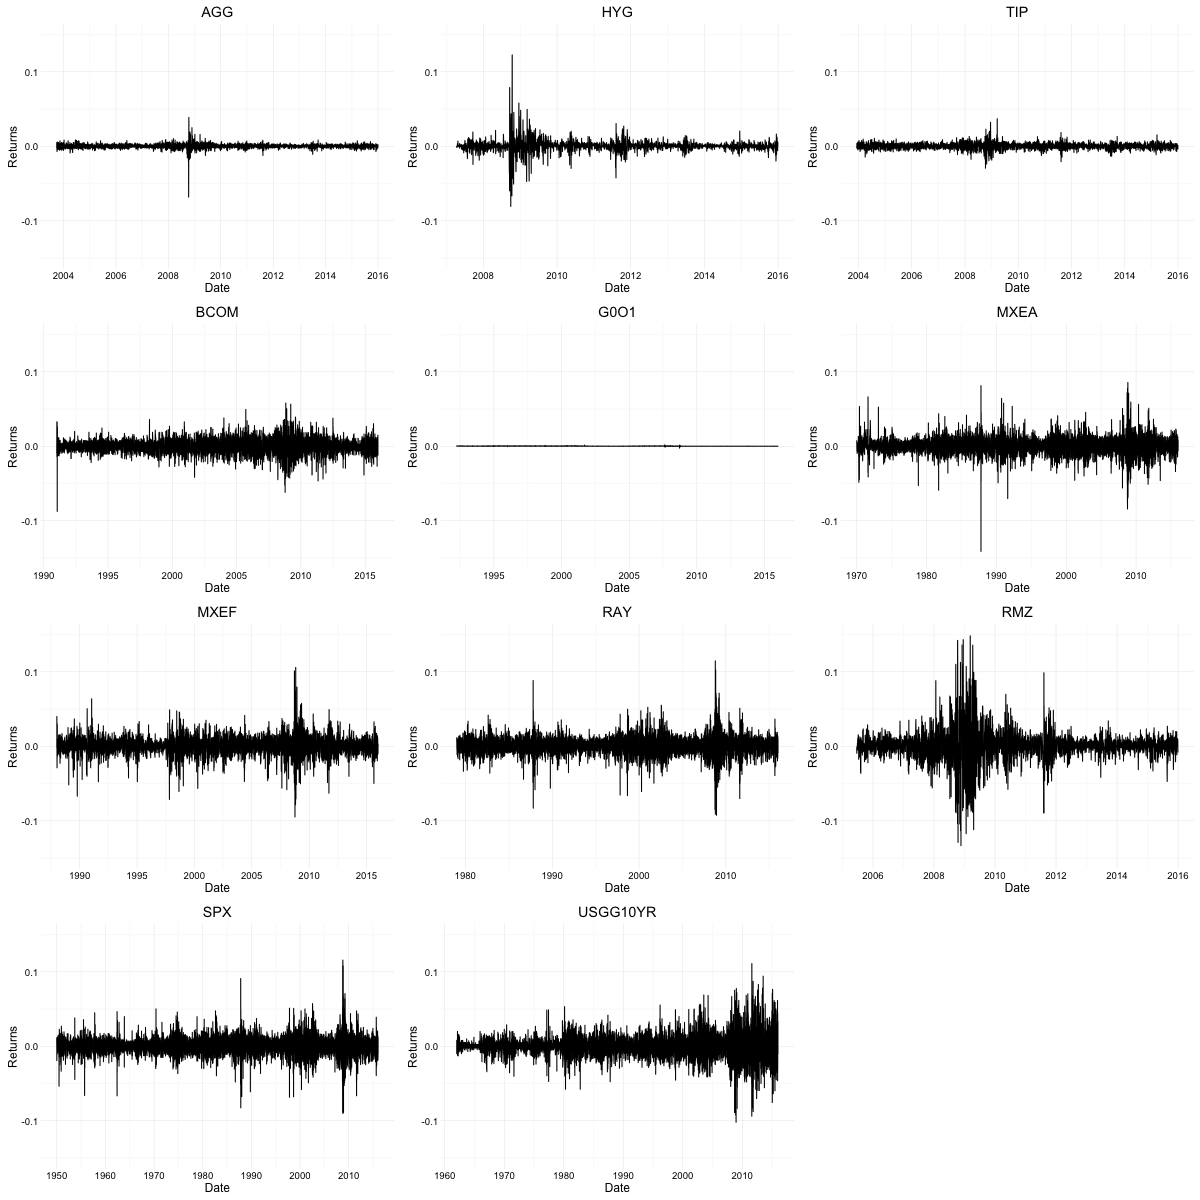
\includegraphics[width=6cm]{../figures/summary_daily/returns}
\label{fig: dailyReturns}
\caption{Daily Returns}
\end{figure}

\end{columns}
\end{frame}

\subsection{Serial Correlation and Risk Measurements under ARIMA Model}
\begin{frame}
\frametitle{$\kappa$(1) and Risk Measurements}
\Fontviii
\begin{columns}[c] % The "c" option specifies centered vertical alignment while the "t" option is used for top vertical alignment

\column{.35\textwidth} % Left column and width
\begin{enumerate}
\item Time series models
\begin{itemize}
\item AR(1)
\item MA(1)
\item ARMA(1,1)
\end{itemize}
\item Risk measurements
\begin{itemize}
\item VaR
\item ES
\item CED
\end{itemize}
\end{enumerate}

\column{.6\textwidth} % Right column and width
\begin{figure}[h]
\centering 
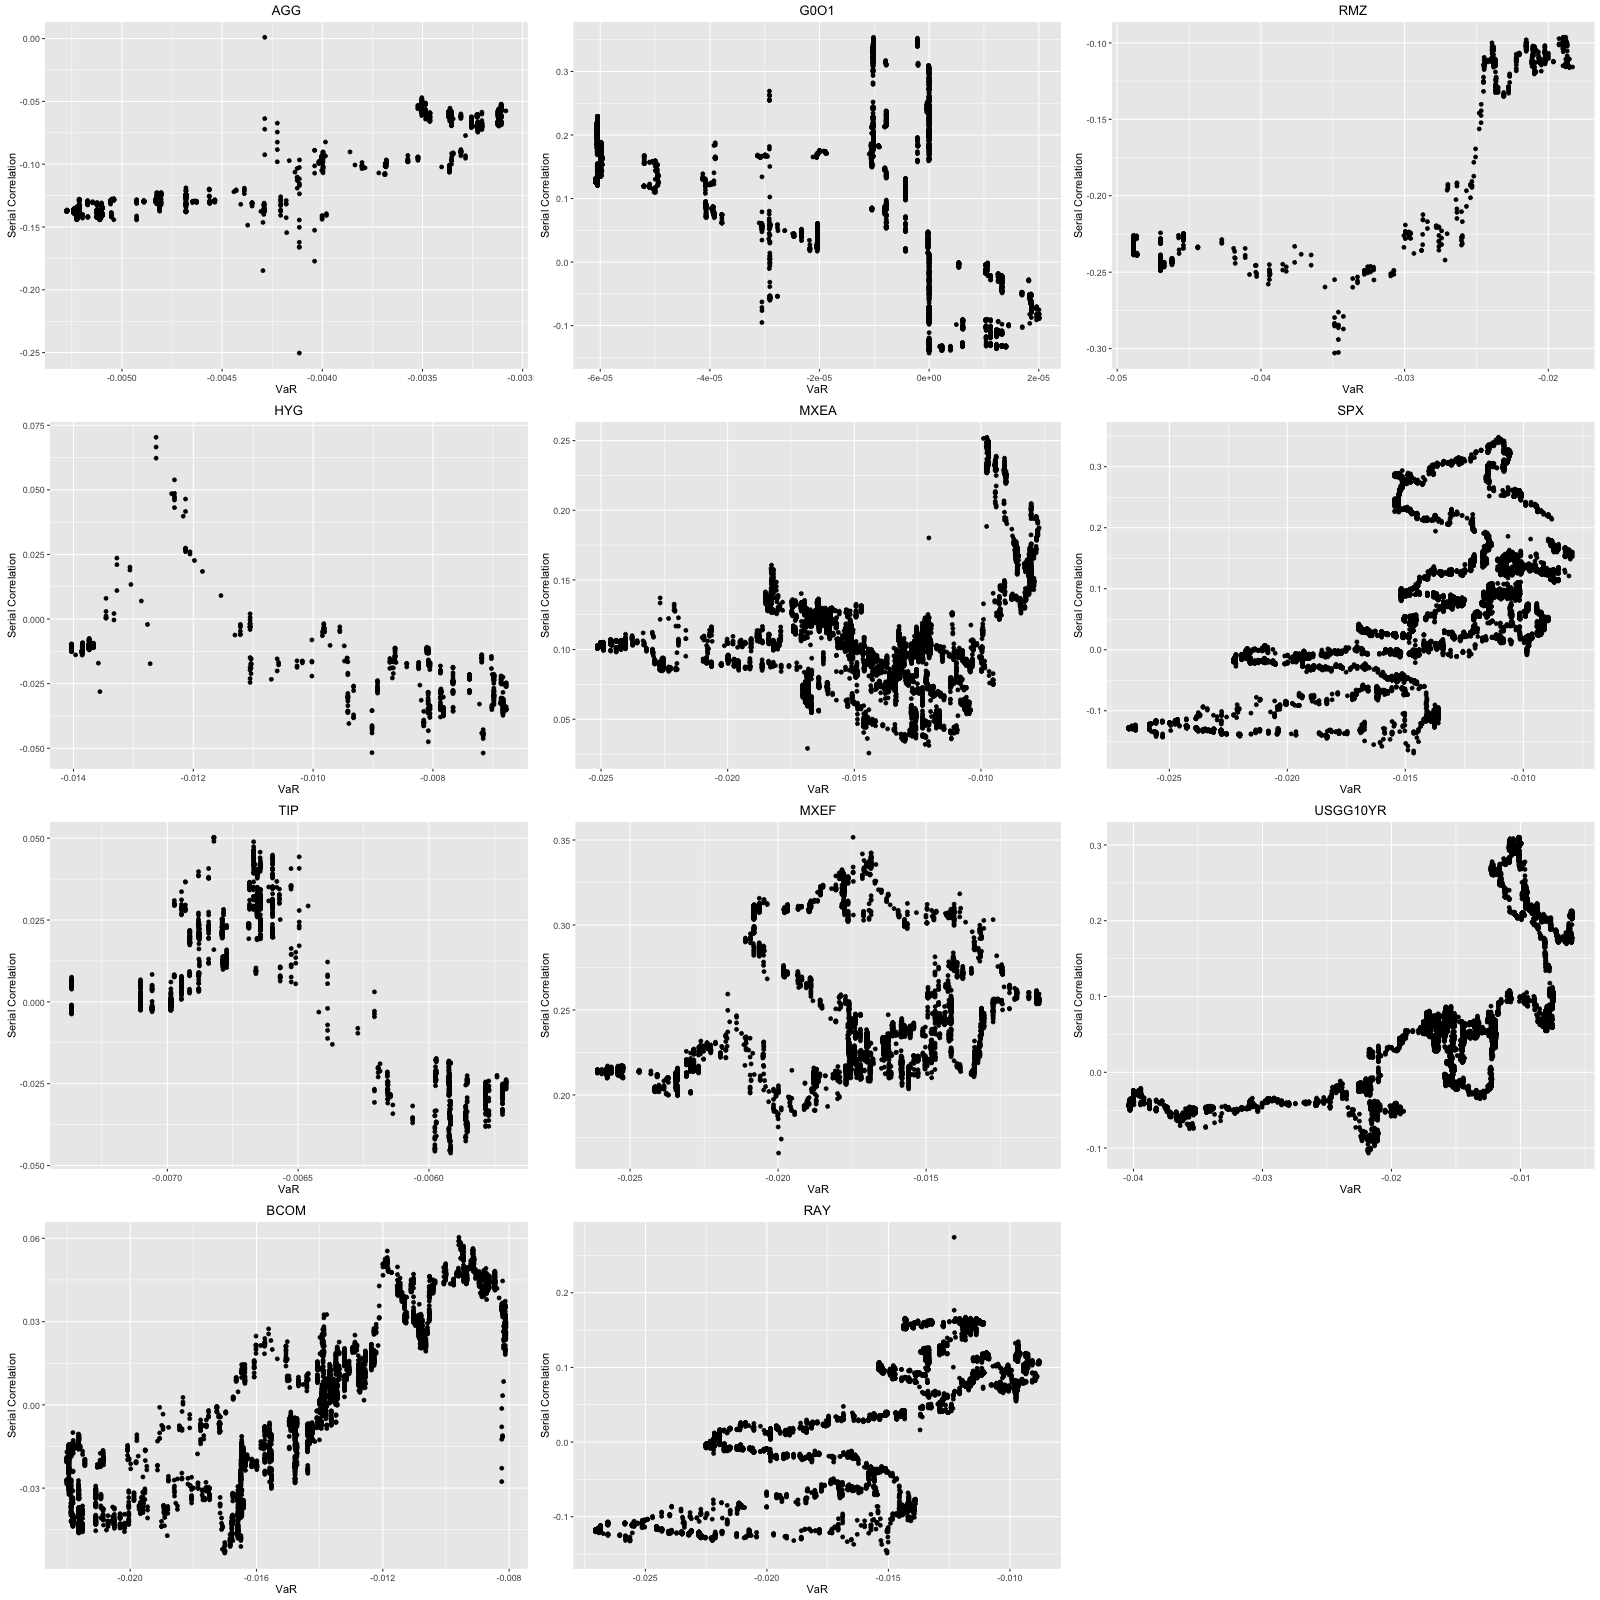
\includegraphics[width=6cm]{../results/SerCol-VaR5yrAR1}
\label{fig:SerCol-VaR5yrAR1}
\caption{AR(1): $\kappa(1)$ versus VaR}
\end{figure}
\end{columns}
\end{frame}


\subsection{Summary of ARMA}
\begin{frame}
\frametitle{ARMA is not enough...}
\Fontviii
\begin{columns}[c]
\column{.35\textwidth} % Left column and width
\begin{enumerate}
\item Inherently non-stationary
\item Clustered Variance
\begin{itemize}
\item GARCH Model
\item Regime Model
\end{itemize}
\end{enumerate}

\column{.6\textwidth} % Right column and width
\begin{figure}[h]
\centering 
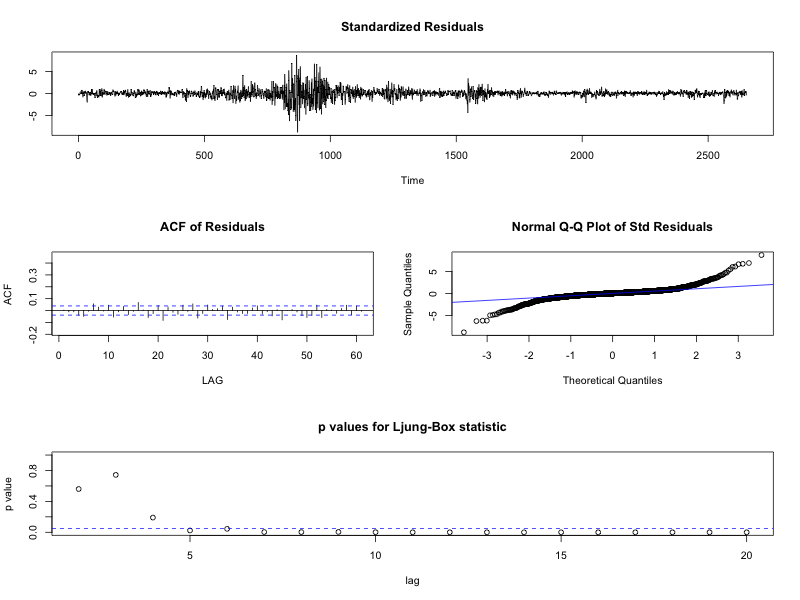
\includegraphics[width=6cm,height = 6cm]{../results/DiagnosticRMZ}
\label{fig: dailyReturns}
\caption{Fit RMZ Data using MA(1)}
\end{figure}

\end{columns}
\end{frame}

%------------------------------------------------
\section{Time Series – GARCH model}
%------------------------------------------------
\subsection{Summary of GARCH Model}
\begin{frame}
\frametitle{Summary of GARCH Model}
\Fontviiii

\begin{table}[!h]
\caption{Best GARCH Model for the residuals after Fitting ARIMA}
\centering 
\begin{tabular}{ | c || r | } 
 \hline
Asset & ARIMA (p,q)+ GARCH(m,n) \\
  \hline \hline
AGG & ARMA(5,5)+GARCH(1,1) \\ 
HYG & ARMA(3,1)+GARCH(1,1) \\ 
TIP &  GARCH(1,1)\\ 
BCOM & GARCH(1,1)\\ 
MXEA & ARMA(2,2)+ GARCH(1,2) \\ 
MXEF & ARMA(4,2) + GARCH(1,1)\\ 
RAY &  ARMA(2,2) + GARCH(1,1)\\ 
RMZ & MA(1) + GARCH(1,1) \\ 
SPX & ARMA(2,2) +GARCH(1,1)\\ 
USGG10YR & GARCH(1,3) \\
 \hline
\end{tabular}
\label{table:BestGarch}
\end{table}
\end{frame}

\subsection{Fit GARCH}
\begin{frame}
\frametitle{RMZ example: Workflow and Diagnostics}
\Fontviii
\begin{columns}[c]
\column{.4\textwidth}
\begin{enumerate}
\item Fit Best ARIMA model, and extract residuals.
\item Select proper GARCH model for the residuals, based on BIC.
\item Check the diagnostic plots
\begin{itemize}
\item Good in general.
\item Heavy Tail.
\end{itemize}
\end{enumerate}
 
 
\column{.6\textwidth} % Right column and width
\begin{figure}[h]
\centering 
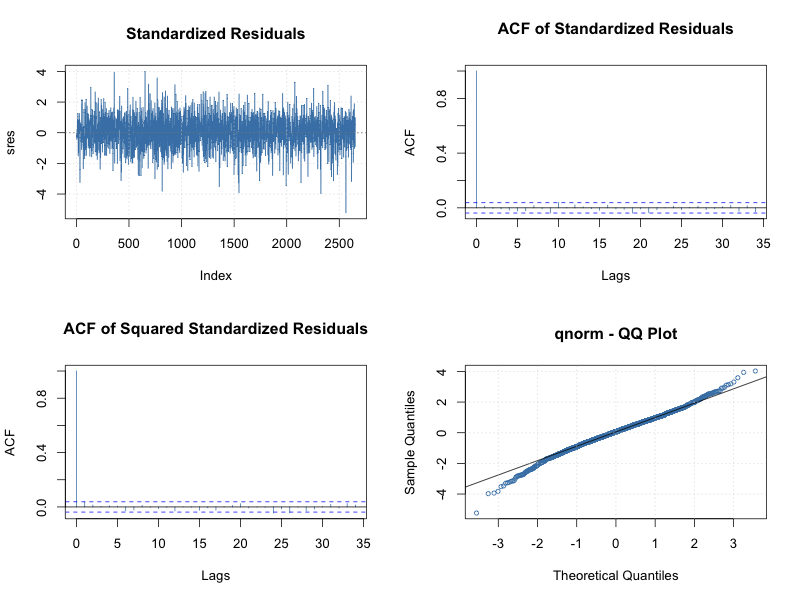
\includegraphics[width=6cm,height = 6cm]{../results/RMZ_GARCH_dig1}
\label{fig:RMZ_GARCH_dig1}
\caption{RMZ example: Diagnostics after Fitting Residual with GARCH(1,1)}
\end{figure}

\end{columns}
\end{frame}

\begin{frame}
\frametitle{RMZ example: Predictions}
\Fontviii
\begin{columns}[c]
\column{.4\textwidth}
\begin{enumerate}
\item Empirical results are similar to the estimation.
\item The second plot give a confident interval for residuals
\item Several steps forward estimation.
\end{enumerate}
 
 
\column{.6\textwidth} % Right column and width
\begin{figure}[h]
\centering 
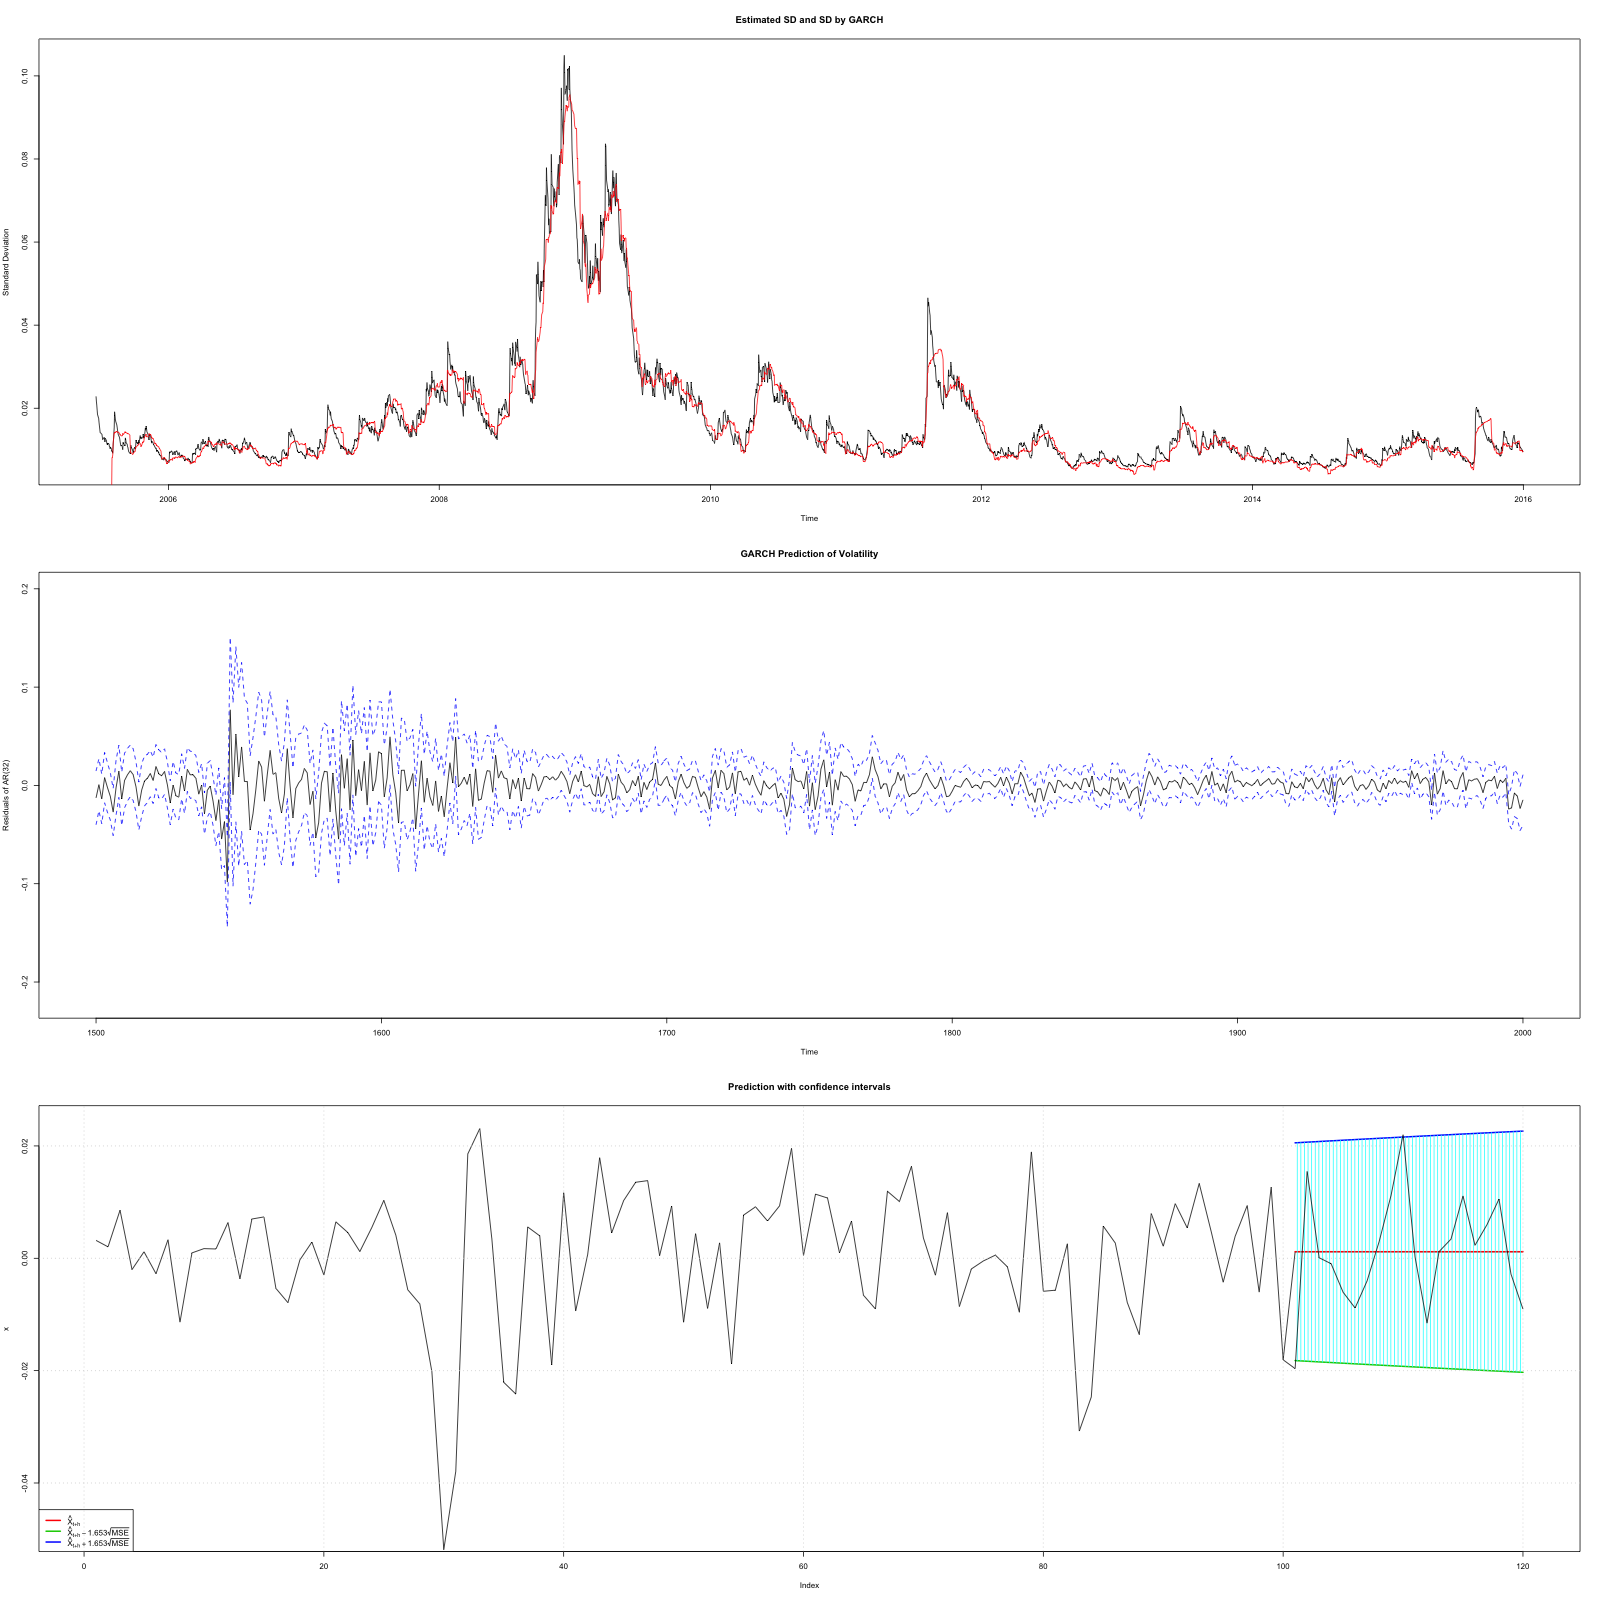
\includegraphics[width=6cm,height = 6cm]{../figures/RMZeg_pred}
\label{fig: dailyReturns}
\caption{RMZ example: Some Prediction Results}
\end{figure}

\end{columns}
\end{frame}

\subsection{Serial Correlation and Risk Measurements}
\begin{frame}
\frametitle{$\kappa(1)$ and CED Using the ``Best" Model}
\Fontviii
\begin{columns}[c]
\column{.4\textwidth}
\begin{enumerate}
\item Almost no pattern there.
\item Correlations are small, and almost negative.
\item Similar to other risk measurement, but less significant
\end{enumerate}
 
 
\column{.6\textwidth} % Right column and width
\begin{figure}[h]
\centering 
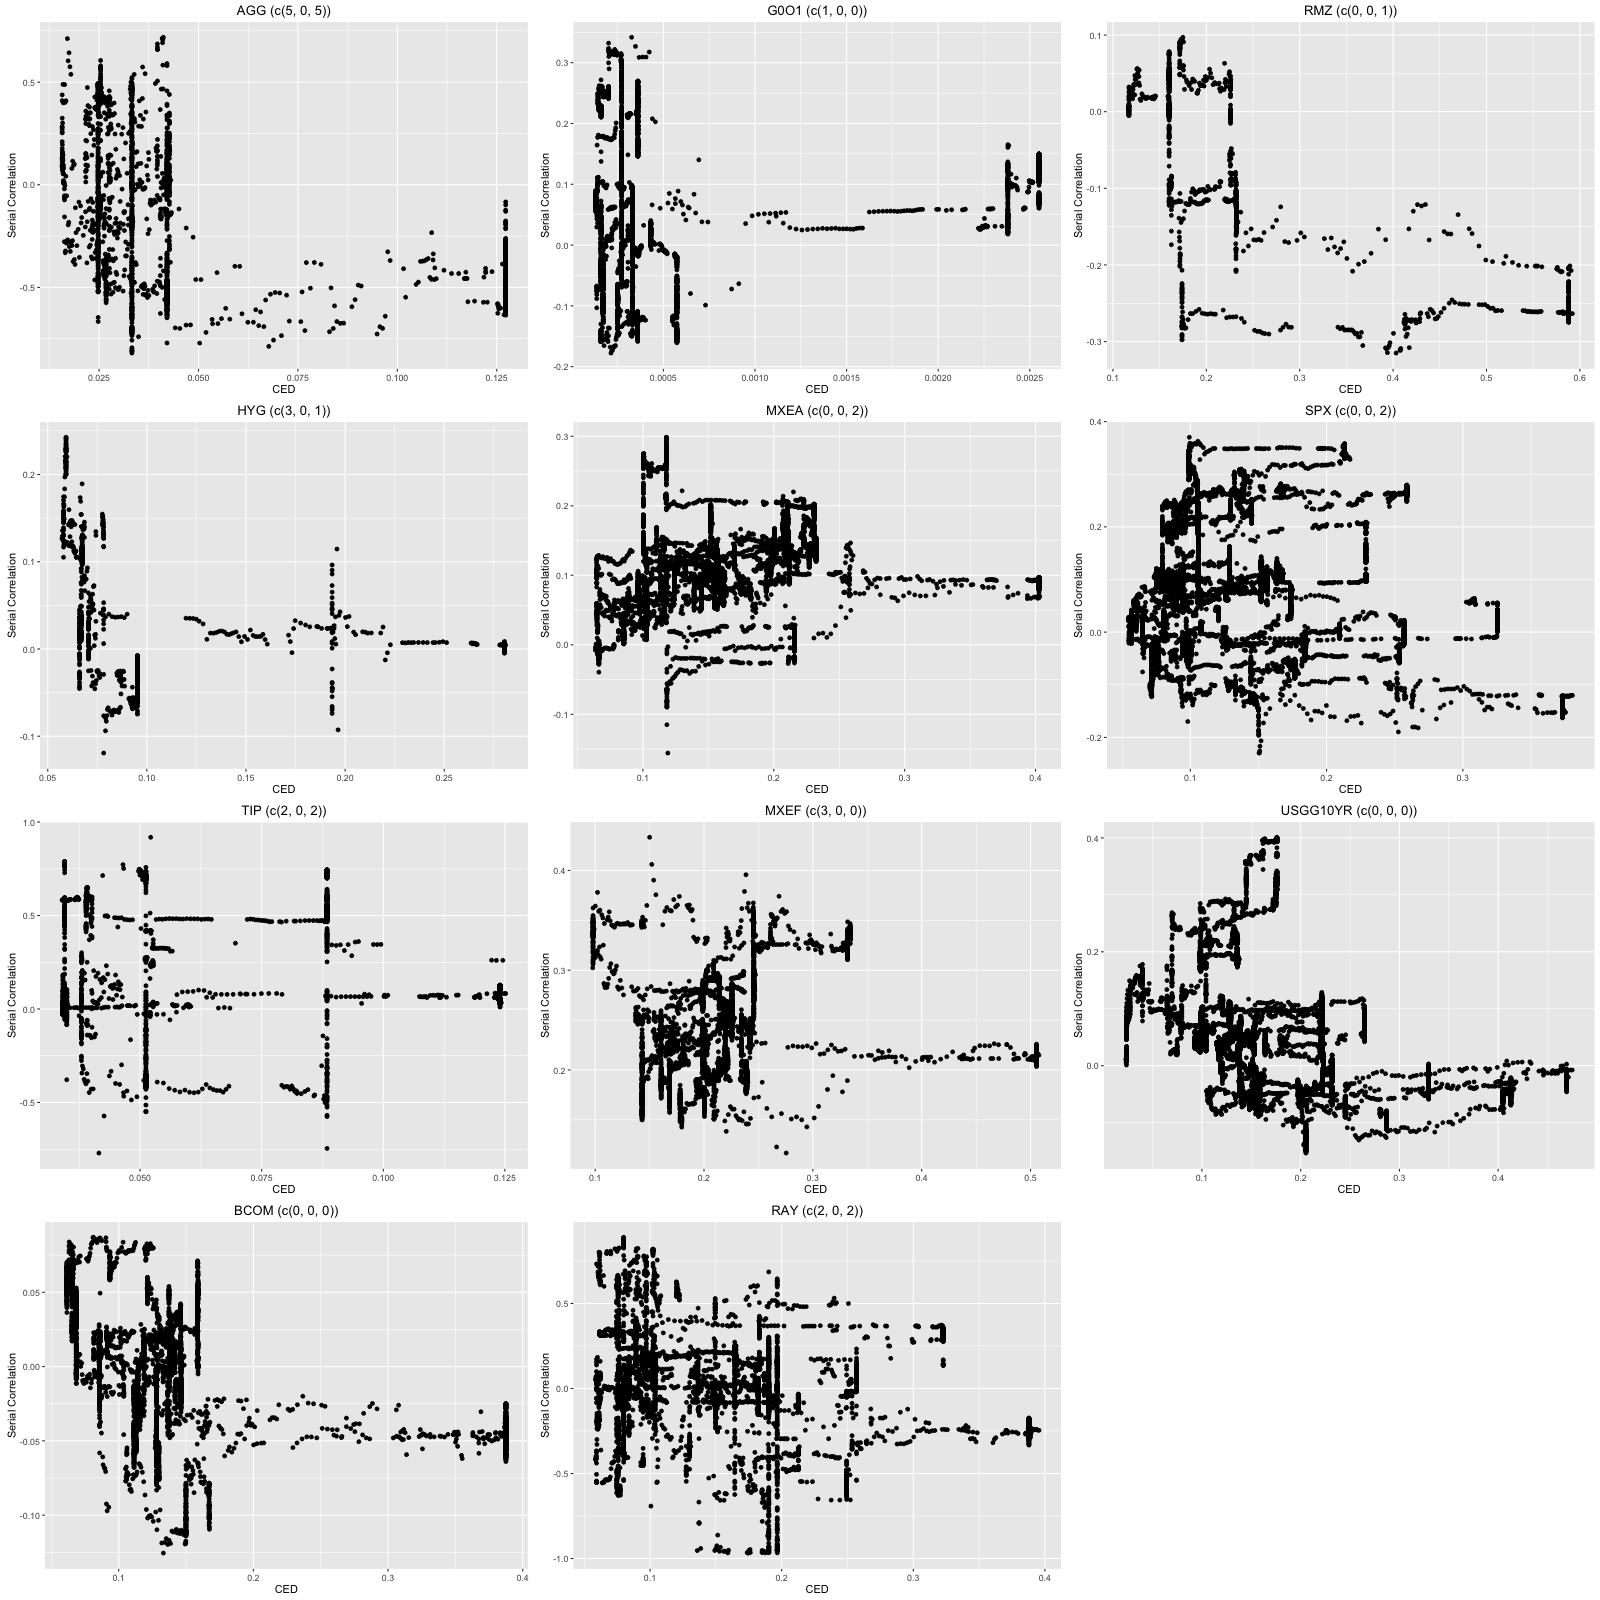
\includegraphics[width=6cm,height = 6cm]{../figures/SerCol-CED3mon2yr}
\label{fig:SerCol-CED3mon2yr}
\caption{$\kappa(1)$ versus CED}
\end{figure}

\end{columns}
\end{frame}
%------------------------------------------------
\section{Analysis of weekly and monthly frequencies}
%------------------------------------------------

%------------------------------------------------
\section{Current work: simulation}
%------------------------------------------------


%------------------------------------------------

\begin{frame}
\Huge{\centerline{The End}}
\end{frame}

%----------------------------------------------------------------------------------------

\end{document} 